\chapter{Sayılabilirlik Aksiyomları}

Sayılabilirlik aksiyomları, bir topolojik uzaydaki ``bilgi''nin sayılabilir büyüklükte
yapılarla tanımlanıp tanımlanamayacağını araştırır.

%-------------------------------------------------------------------
\section{Konu}

\subsection{Sayılabilirlik Aksiyomları}

\begin{table}[h]
\centering
\begin{tabular}{ll}
\toprule
\textbf{Aksiyom} & \textbf{Tanım} \\
\midrule
Birinci sayılabilir & Her $x \in X$ için sayılabilir yerel baz \\
İkinci sayılabilir & Tüm topoloji için sayılabilir global baz \\
Ayrılabilir & Sayılabilir yoğun alt küme: $\overline{D} = X$ \\
Lindelöf & Her açık örtünün sayılabilir alt-örtüsü \\
\bottomrule
\end{tabular}
\caption{Sayılabilirlik aksiyomları}
\end{table}

\textbf{Sıralamalar:}
\begin{itemize}
  \item $2^{\text{nd}}$ sayılabilir $\Rightarrow$ $1^{\text{st}}$ sayılabilir
  \item $2^{\text{nd}}$ sayılabilir $\Rightarrow$ ayrılabilir $\wedge$ Lindelöf
  \item Metrik $\Rightarrow$ $1^{\text{st}}$ sayılabilir
  \item Ayrılabilir metrik $\Rightarrow$ $2^{\text{nd}}$ sayılabilir
\end{itemize}

\begin{figure}[ht]
  \centering
  \begin{tikzpicture}[font=\small, node distance=10mm,
    aks/.style={draw, rounded corners, fill=blue!6, inner sep=5pt, align=center}]
  \node[aks] (sc) {2.\ sayılabilir\\ (sayılabilir baz)};
  \node[aks, above right=10mm and 16mm of sc] (fc) {1.\ sayılabilir\\ (sayılabilir yerel baz)};
  \node[aks, right=24mm of sc] (sep) {ayrılabilir\\ (yoğun say.\ alt küme)};
  \node[aks, below right=10mm and 16mm of sc] (lin) {Lindelöf\\ (say.\ alt-örtü)};
  \draw[-{Stealth[length=2.6mm]}, thick] (sc) -- (fc);
  \draw[-{Stealth[length=2.6mm]}, thick] (sc) -- (sep);
  \draw[-{Stealth[length=2.6mm]}, thick] (sc) -- (lin);
  \node[aks, fill=green!7, left=22mm of sc, align=center] (met) {metrik\\ uzay};
  \draw[-{Stealth[length=2.6mm]}, thick] (met) -- (fc.west);
  \draw[red!70!black, -{Stealth[length=2.2mm]}, dashed]
    (fc.east) to[bend left=22] node[right=2pt, font=\scriptsize, align=center]
    {tersi geçmez:\\ Sorgenfrey doğrusu\\ (1., ayrıl., Lindelöf\\ ama 2.\ sayılabilir değil)} (sep.east);
\end{tikzpicture}

  \caption{Sayılabilirlik aksiyomları arasındaki implikasyonlar: düz oklar
    $2^{\text{nd}}$ sayılabilirden $1^{\text{st}}$ sayılabilir, ayrılabilir ve
    Lindelöf'e gider; metrik uzaylar $1^{\text{st}}$ sayılabilirdir. Kesikli
    kırmızı ok terslerin geçmediği kanonik karşı-örneği (Sorgenfrey doğrusu)
    işaretler.}
  \label{fig:ch09:implikasyon}
\end{figure}

\begin{sezgi}
Sayılabilirlik aksiyomları, bir uzayı ``sayılabilir bir sözlükle'' anlatabilme
sorusudur. $2^{\text{nd}}$ sayılabilirlik uzayın \emph{tüm} açıklarını sayılabilir
bir baz listesinden kurar --- tek bir küresel sözlük. $1^{\text{st}}$ sayılabilirlik
ise yalnızca \emph{her nokta için ayrı} sayılabilir bir komşuluk listesi ister ---
yerel sözlükler. Küresel liste her noktaya yerel liste verdiğinden
$2^{\text{nd}}\Rightarrow 1^{\text{st}}$; tersi her zaman doğru değildir.
\end{sezgi}

\begin{figure}[ht]
  \centering
  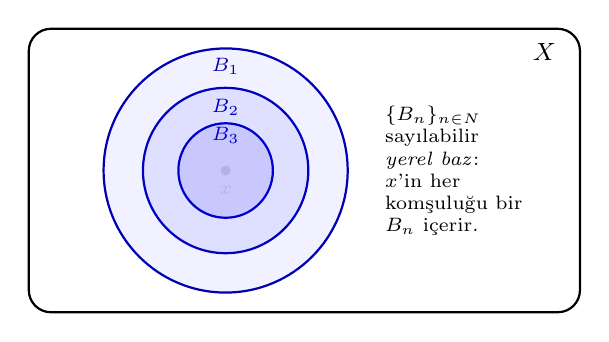
\begin{tikzpicture}[font=\small]
  % carrier box
  \draw[rounded corners=8pt, thick] (-0.4,-1.4) rectangle (6.6,2.2);
  \node at (6.15,1.9) {$X$};
  % nested neighborhoods around x  (countable local base)
  \fill (2.1,0.4) circle (1.8pt) node[below=2pt, font=\scriptsize] {$x$};
  \draw[blue!70!black, thick, fill=blue!12, fill opacity=0.45] (2.1,0.4) circle (1.55);
  \draw[blue!75!black, thick, fill=blue!18, fill opacity=0.55] (2.1,0.4) circle (1.05);
  \draw[blue!80!black, thick, fill=blue!26, fill opacity=0.65] (2.1,0.4) circle (0.6);
  \node[blue!70!black, font=\scriptsize] at (2.1,1.72) {$B_1$};
  \node[blue!75!black, font=\scriptsize] at (2.1,1.2)  {$B_2$};
  \node[blue!80!black, font=\scriptsize] at (2.1,0.85) {$B_3$};
  \node[align=left, anchor=west, font=\scriptsize] at (4.0,0.4)
    {$\{B_n\}_{n\in\mathbb{N}}$\\ sayılabilir\\ \emph{yerel baz}:\\ $x$'in her\\ komşuluğu bir\\ $B_n$ içerir.};
\end{tikzpicture}

  \caption{Bir $x$ noktası çevresinde iç içe küçülen $B_1\supseteq B_2\supseteq B_3$
    komşulukları: sayılabilir bir \emph{yerel baz}. $x$'in her komşuluğu bir $B_n$
    içerir.}
  \label{fig:ch09:yerelbaz}
\end{figure}

\begin{karsiornek}
\textbf{Sorgenfrey doğrusu.} $[a,b)$ biçimli yarı-açık aralıklarla üretilen
Sorgenfrey doğrusu $1^{\text{st}}$ sayılabilir, ayrılabilir \emph{ve} Lindelöf'tür
ama $2^{\text{nd}}$ sayılabilir \emph{değildir}. Her $x$ için
$\{[x, x+1/n) : n\in\mathbb{N}\}$ sayılabilir yerel baz verir; $\mathbb{Q}$
yoğundur. Ama herhangi bir baz, her $x$ için tam $x$'te başlayan bir eleman
içermek zorundadır; farklı $x$'ler farklı eleman gerektirir, dolayısıyla baz en
az continuum büyüklükte --- sayılamaz. Yani
``$2^{\text{nd}}\Leftarrow 1^{\text{st}}\wedge$ ayrılabilir $\wedge$ Lindelöf''
çıkarımı geçersizdir. \texttt{sorgenfrey\_line\_like()} ile test edilir.
\end{karsiornek}

%-------------------------------------------------------------------
\section{Teoremler}

\begin{theorem}
$2^{\text{nd}}$ sayılabilir $\Rightarrow$ ayrılabilir $\wedge$ Lindelöf.
\begin{proof}[İspat eskizi]
$\mathcal{B}=\{B_n\}$ sayılabilir baz olsun. \textbf{Ayrılabilir:} her boş olmayan
$B_n$'den bir $d_n$ seç; $D=\{d_n\}$ sayılabilirdir ve her boş olmayan açık $U$ bir
$B_n\subseteq U$ içerdiğinden $d_n\in U\cap D$ --- yani $\overline{D}=X$.
\textbf{Lindelöf:} keyfi açık örtü $\{U_\alpha\}$'da kullanılan her noktayı içeren
bir $B_n$'i, onu kapsayan bir $U_\alpha$ ile eşle; kullanılan $B_n$'ler sayılabilir
olduğundan seçilen $U_\alpha$'lar sayılabilir bir alt-örtü verir.
\end{proof}
\end{theorem}

\begin{theorem}
Metrik uzay $\Rightarrow$ $1^{\text{st}}$ sayılabilir.
\begin{proof}[Kanıt İskeleti]
Her $x$ için $\{B(x, 1/n) : n \in \mathbb{N}\}$ sayılabilir yerel bazdır.
\end{proof}
\end{theorem}

\begin{theorem}
Ayrılabilir + metrik $\Rightarrow$ $2^{\text{nd}}$ sayılabilir.
\begin{proof}[Kanıt İskeleti]
$D \subseteq X$ yoğun sayılabilir; $\{B(d, 1/n) : d \in D,\, n \in \mathbb{N}\}$ sayılabilir bazdır.
\end{proof}
\end{theorem}

\begin{theorem}[Sorgenfrey Karşı Örneği]
Sorgenfrey doğrusu ayrılabilir ve Lindelöf'tür ama $2^{\text{nd}}$ sayılabilir
değildir. (Yukarıdaki karşı-örnek kutusuna bakın.)
\end{theorem}

\begin{theorem}[Sayılamaz Ayrık Uzay --- İkinci Karşı Örnek]
Sayılamaz taşıyıcı üzerindeki ayrık topoloji $1^{\text{st}}$ sayılabilirdir ama
ayrılabilir, Lindelöf ve $2^{\text{nd}}$ sayılabilir \emph{değildir}.
\begin{proof}[İspat eskizi]
Her $\{x\}$ açık olduğundan $\{\{x\}\}$ tek elemanlı yerel bazdır
($1^{\text{st}}$ sayılabilir). Yoğun bir küme her $\{x\}$'i kesmek zorunda olduğundan
taşıyıcının tamamını içermelidir; taşıyıcı sayılamaz olduğundan ayrılabilir değildir.
$\{\{x\}\}_{x\in X}$ örtüsünün sayılabilir alt-örtüsü yoktur (Lindelöf değil) ve her
baz tüm $\{x\}$'leri içermek zorunda olduğundan sayılamaz ($2^{\text{nd}}$ sayılabilir
değil). \texttt{uncountable\_discrete\_space()} ile doğrulanır.
\end{proof}
\end{theorem}

\begin{figure}[ht]
  \centering
  \begin{tikzpicture}[font=\small]
  % real line
  \draw[thick, -{Stealth[length=2.4mm]}] (-0.4,0) -- (8.6,0) node[right] {$\mathbb{R}$};
  \foreach \x in {0,1,2,3,4,5,6,7,8}
    \draw[thick] (\x,-0.08) -- (\x,0.08);
  \node[font=\scriptsize] at (0,-0.32) {$0$};
  \node[font=\scriptsize] at (4,-0.32) {$4$};
  \node[font=\scriptsize] at (8,-0.32) {$8$};
  % sample rational points (dense countable subset Q)
  \foreach \x in {0.3,0.7,1.25,1.6,2.1,2.55,3.0,3.4,3.85,4.3,4.7,5.2,5.65,6.1,6.5,6.95,7.4,7.8}
    \fill[red!75!black] (\x,0) circle (1.3pt);
  % a target open interval
  \draw[blue!70!black, thick] (4.95,0.45) -- (5.95,0.45);
  \draw[blue!70!black, thick] (4.95,0.35) -- (4.95,0.55);
  \draw[blue!70!black, thick] (5.95,0.35) -- (5.95,0.55);
  \node[blue!70!black, font=\scriptsize] at (4.55,0.78) {$(a,b)$};
  \draw[red!75!black, -{Stealth}, thick] (5.65,1.45) -- (5.45,0.55);
  \node[red!75!black, font=\scriptsize, align=center] at (6.35,1.45) {içinde bir\\ $q\in\mathbb{Q}$ var};
  \node[align=center, font=\scriptsize] at (4.0,-1.0)
    {$\mathbb{Q}$ (kırmızı noktalar) sayılabilir ve $\overline{\mathbb{Q}}=\mathbb{R}$:\\
     her boş olmayan açık aralık bir rasyonel içerir $\Rightarrow$ $\mathbb{R}$ ayrılabilirdir.};
\end{tikzpicture}

  \caption{Ayrılabilirlik: $\mathbb{Q}$ (kırmızı noktalar) sayılabilirdir ve
    $\overline{\mathbb{Q}}=\mathbb{R}$. Her boş olmayan açık aralık $(a,b)$ bir
    rasyonel içerdiğinden $\mathbb{R}$ ayrılabilirdir.}
  \label{fig:ch09:ayrilabilirlik}
\end{figure}

%-------------------------------------------------------------------
\section{Algoritmalar}

\subsection{Sonlu Uzayda Sayılabilirlik}

Sonlu uzayda her aksiyom trivially sağlanır. $O(1)$.

\subsection{Sonsuz Uzayda: Tag-Tabanlı Çıkarım}

pytop sembolik uzaylarda tag koridorlarından sayılabilirlik çıkarır:
\begin{itemize}
  \item \texttt{'second\_countable'} $\in$ tags $\Rightarrow$ tüm aksiyomlar
  \item \texttt{'metric'} $\wedge$ \texttt{'separable'} $\Rightarrow$ \texttt{'second\_countable'}
\end{itemize}

%-------------------------------------------------------------------
\section{pytop API}

\begin{lstlisting}[language=Python]
from pytop import (
    is_first_countable,
    is_second_countable,
    is_separable,
    is_lindelof,
)
# Yardimcilar:
from pytop import countability_report, is_dense_subset
\end{lstlisting}

\texttt{countability\_report(space)} dört aksiyomu bir \texttt{dict} içinde
toplar; \texttt{is\_dense\_subset(space, subset)} ayrılabilirliği somut bir
tanıkla gösterir.

%-------------------------------------------------------------------
\section{Örnekler}

\subsection*{Örnek 5.1 — Gerçek Doğru: Tüm 4 Aksiyom}

\begin{lstlisting}[language=Python]
rl = real_line_metric()
print("1st countable?", is_first_countable(rl).status)
print("2nd countable?", is_second_countable(rl).status)
print("separable?", is_separable(rl).status)
print("lindelof?", is_lindelof(rl).status)
\end{lstlisting}

\begin{verbatim}
1st countable?  true
2nd countable?  true
separable?      true
lindelof?       true
\end{verbatim}

\subsection*{Örnek 5.5 — Sorgenfrey Doğrusu: 2nd Countable $\times$}

\begin{lstlisting}[language=Python]
from pytop import sorgenfrey_line_like
sl = sorgenfrey_line_like()
print("1st countable?", is_first_countable(sl).status)
print("2nd countable?", is_second_countable(sl).status)
print("separable?", is_separable(sl).status)
\end{lstlisting}

\begin{verbatim}
1st countable?   true
2nd countable?   false
separable?       true
\end{verbatim}

\subsection*{Örnek 5.6 — Toplu Rapor + Yoğunluk Tanığı}

\begin{lstlisting}[language=Python]
from pytop import countability_report, is_dense_subset
from pytop import sorgenfrey_line_like, discrete_topology

rep = countability_report(sorgenfrey_line_like())
for key in ['first_countable','second_countable','separable','lindelof']:
    print(f"  {key:<17}: {rep[key].status}")

d = discrete_topology(1, 2, 3)
print("dense {1,2,3}?", is_dense_subset(d, {1, 2, 3}).status)
print("dense {1,2}?  ", is_dense_subset(d, {1, 2}).status)
\end{lstlisting}

\begin{verbatim}
  first_countable  : true
  second_countable : false
  separable        : true
  lindelof         : true
dense {1,2,3}? true
dense {1,2}?   false
\end{verbatim}

\subsection*{Örnek 5.7 — Sayılamaz Ayrık Uzay: İkinci Karşı Örnek}

\begin{lstlisting}[language=Python]
from pytop import uncountable_discrete_space
from pytop import (is_first_countable, is_second_countable,
                   is_separable, is_lindelof)

u = uncountable_discrete_space()
print("1st countable?", is_first_countable(u).status)
print("2nd countable?", is_second_countable(u).status)
print("separable?    ", is_separable(u).status)
print("lindelof?     ", is_lindelof(u).status)
\end{lstlisting}

\begin{verbatim}
1st countable? true
2nd countable? false
separable?     false
lindelof?      false
\end{verbatim}

Her tekil $\{x\}$ açık olduğundan yerel baz tek elemanlıdır ($1^{\text{st}}$
sayılabilir), ama yoğun sayılabilir alt küme ve sayılabilir alt-örtü yoktur.

%-------------------------------------------------------------------
\section{Alıştırmalar}

\subsection*{Kodlama}

\begin{enumerate}[label=K\arabic*.]
\item \texttt{finite\_chain\_space(5)} üzerinde \texttt{is\_first\_countable} ve
      \texttt{is\_second\_countable} hesaplayın.
\item İki noktalı ayrık ve indiscrete uzaylar üzerinde \texttt{is\_separable} karşılaştırın.
\item \texttt{integers\_discrete()} için $2^{\text{nd}}$ sayılabilir mi?
\item \texttt{uncountable\_discrete\_space()} üzerinde dört aksiyomu
      \texttt{countability\_report} ile hesaplayıp \texttt{integers\_discrete()}
      ile karşılaştırın. Hangi aksiyom(lar)da ayrışıyorlar?
      \ipucu{Fark, taşıyıcının sayılabilir olup olmamasındadır.}
\end{enumerate}

\subsection*{Teori}

\begin{enumerate}[label=T\arabic*.]
\item $2^{\text{nd}}$ sayılabilir $\Rightarrow$ ayrılabilir olduğunu ispatlayın.
\item Sorgenfrey doğrusunun $2^{\text{nd}}$ sayılabilir olmadığını gösterin.
\item ``$1^{\text{st}}$ sayılabilir $\Rightarrow$ ayrılabilir'' çıkarımının yanlış
      olduğunu bir karşı-örnekle gösterin.
      \ipucu{Sayılamaz ayrık uzay; yoğun küme her $\{x\}$'i kesmek zorundadır.}
\end{enumerate}
